\section{Digital Representation of Numbers}
\thispagestyle{plain}

In C, \mintinline{C}{int x = 100 * 200 * 300 * 400;} will surprisingly yield $-1894967296$ (for a 32-bit integer
representation) (\textit{overflow}), \mintinline{C}{float f1 = (2.3 + 1e20) - 1e20;} yields $0.0$ (\textit{round-off-error}) but
\mintinline{C}{float f2 = 2.3 + (1e20 - 1e20);} correctly gives $2.3$.

We want to understand and mitigate such caveats of arithmetic on computers, where we want quick calculations while also
using as little storage as possible - simulations can quickly become big in storage (e.g. lots of particles).

Further details can be found in \cite{higham02} and \cite{bryant2011computer}.

\subsection{Integer Arithmetic}

In C, integers ($\in \mathbb{Z}$) are stored as fixed-size bit-sequences. The respective size
dictates a range. C provides both unsigned and signed integer types, with negative numbers
in the signed case represented using \textit{two's-complements}.

\subsubsection{Unsigned integers}
For a bit-vector $\vec{x} = [x_{\omega-1},x_{\omega-2},\dots,x_0]$ the unsigned conversion is

\begin{equation}
    B2U_{\omega} := \sum_{i=0}^{\omega-1} x_i 2^i
\end{equation}

(illustrated in figure \ref{fig:unchar}) and the range is $0,\dots,2^\omega - 1$. In case of overflow in operations, the overflow is truncated
in the most significant bits (see figure \ref{fig:uncharadd}). As $B2U_{\omega}[x_{\omega-1},x_{\omega-2},\dots,x_0] \mod 2^k = 
B2U_{\omega}[x_{k-1},x_{k-2},\dots,x_0]$ we effectively store $\text{arithmetic result}\mod 2^\omega$.

$x_{\omega-1}$ is called most significant bit (MSB) and $x_0$ least significant bit (LSB).

\problem{When the result of an arithmetic operation exceeds the range of an integer type, unexpected results occur (overflow) (and also underflow in the signed case)}

\begin{figure}[!htb]
 \centering
 \includesvg[width=0.9\textwidth]{figures/unchar.svg}\hfill
 \caption{Example of an unsigned char in C.}
 \label{fig:unchar}
\end{figure}

\begin{figure}[!htb]
    \centering
    \includesvg[width=0.9\textwidth]{figures/uncharadd.svg}\hfill
    \caption{Example of unsigned char overflow.}
    \label{fig:uncharadd}
\end{figure}

\subsubsection{Two's complement for negative numbers}
Note that addition of integers by bitwise addition with carry-on is very fast.

\redbox{\textbf{Why can't we just let the MSB encode the sign?:} A representation of the form
\begin{equation}
    B2S_\omega(\vec{x}) := (-1)^{x_{\omega - 1}} \cdot \sum_{i=0}^{\omega-2} x_i 2^i
\end{equation}
(sign magnitude) has the disadvantage, that normal bitwise addition with carry-on does not work. Also, zero is
encoded twice, as $\pm 0$.
}

\greenbox{\textbf{Idea of the two's-complement:} The MSB flags the sign in $\vec{x} = [x_{\omega-1},x_{\omega-2},\dots,x_0]$ by 
having a weighting factor $-2^{\omega-1}$
\begin{equation}
    B2T_\omega(\vec{x}) := -x_{\omega-1} 2^{\omega-1} + \sum_{i=0}^{\omega-2} x_i 2^i
\end{equation}
Carry-on to the $\omega$-th bit in addition is again ignored. As we really just have to add positive numbers in bits
$x_0$ to $x_{\omega-2}$ with correct sign-switch by carry-on, no special handling is necessary (see figure \ref{fig:tcompl}). The range is $-2^{\omega-1} \dots 2^{\omega-1} - 1$.
}
From an unsigned int to the two's complement and vice versa we can get by
\begin{enumerate}
    \item invert all bits
    \item add $+1$ to the result\footnote{These rules intuitively follow from the constraint, that bitwise addition with carry-on of $-u$ and $u$ should result in an all-zero bitvector. Adding a bitvector to its inverted self results in an all-1 bitvector, adding one more then results in all zeros, as the last carry-on is discarded.}
\end{enumerate}
If we want $\vec{x}$ with $B2T_\omega(\vec{x}) = -u$ then the bits following the MSB must encode $k$ with $-u = -2^{\omega-1} + k$,
so the encoded unsigned number must be $B2T_\omega(\vec{x}) = \explain{2^{\omega-1}}{\text{sign bit}} + k = 2^{\omega} - u$ - a \textit{two's complement}.

\begin{figure}[!htb]
 \centering
 \includesvg[width=0.9\textwidth]{figures/tcompl.svg}\hfill
 \caption{Illustration of the defining feature of the two's complement - addition is simple.}
 \label{fig:tcompl}
\end{figure}


\subsubsection{Integer types in C}

Some common integer types with respective minimum sizes are given in table \ref{tab:inttypes}.

\begin{table}[!htb]
    \centering
    \begin{tabular}{l|l}
        Type & Minimum Size $\omega$ \\
        \hline
        \mintinline{C}{char} & 8 bits \\
        \mintinline{C}{short} & 16 bits\\
        \mintinline{C}{int} & 16 bits\\
        \mintinline{C}{long} & 32 bits\\
        \mintinline{C}{long long} & 64 bits\\
    \end{tabular}
    \caption{Common integer types in C, signed ranges are $-2^{\omega-1} \dots 2^{\omega-1} - 1$, unsigned ranges are $0 \dots 2^\omega - 1$.}
    \label{tab:inttypes}
\end{table}

\problem{Using unsigned can come with unexpected results, when being cast from a negative number. E.g. \mintinline{C}{unsigned int x = -1;} will result in $2^{32} - 1$ in a 32-bit system (the two's complement is read as if an unsigned representation).
More deviously, $-1 < 0U$ will evaluate to false, as all integers in a comparison are cast to unsigned, when one of them is unsigned.}

\subsubsection{Byte Ordering in Storage: Big and Little Endian}
Bytes of e.g. a multi-byte integer can be stored from most significant byte to least significant byte (big endian) or vice versa (little endian), see figure \ref{fig:endian}.

\begin{figure}[!htb]
 \centering
 \includesvg[width=0.9\textwidth]{figures/endian.svg}\hfill
 \caption{Big and Little Endian.}
 \label{fig:endian}
\end{figure}

\subsubsection{Properties and Caveats of Integer Arithmetic}
Typical problems in integer arithmetic are overflow, integer division, the modulo operation and implicit type conversion.
\redbox{\textbf{Overflow:} The respective integer ranges have finite ranges, overflow in arithmetic operations is cut-off. We must choose a type
with sufficient range - mind that choosing types with too large of a footprint (e.g. always long) wastes storage and compute.\par
\textit{Example I:} In \mintinline{C}{char c = 100 * 4; // range -128 to 127} the result is $-112$ as $400$ in bits is $0001 1001 0000$ where a cut-off to one byte means $1001 0000$ so $-2^7+2^4 = -128 + 16 = -112$.\par
\textit{Example II:} For \mintinline{C}{int a = -1 * pow(2,31); int b = 10;} we have $a<b$ but not $a-b<0$ (for char the behavior is a bit different as up to int there is
implicit type conversion.)
}

\redbox{\textbf{Integer division:} All decimal places are truncated, so 
$$5/3 = 1; -5/3 = -1; 5/-3 = -1$$
}

\redbox{\textbf{Modulo operation:} The modulus in C is defined as $n\%m = n - (n/m)m$ so 
$$5\%3 = 2; -5\%3 = -2; 5\%-3 = -2$$
}

\redbox{\textbf{Implicit type conversion:} In C, the type can implicitly be converted up to unsigned int, which can avoid overflow, as illustrated in table \ref{tab:type_conversion}.
}
\begin{table}[!htb]
    \centering
    \begin{tabular}{p{0.3\textwidth}|p{0.3\textwidth}|p{0.3\textwidth}}
        \textcolor{green1}{implicit type conversion up to int can be helpful} & \textcolor{red1}{mind its only up to int} & \textcolor{green1}{explicit type consversion} \\
        \hline
        \begin{minipage}[t]{0.3\textwidth}
        \begin{minted}[frame=single, obeytabs=true, tabsize=1, breaklines, numbersep=-10pt, gobble=2]{C}
    char a,b;
    a = 100;
    b = 4;
    int c = a * b; // 400
        \end{minted}
        \end{minipage}
        &
        \begin{minipage}[t]{0.3\textwidth}
        \begin{minted}[frame=single, obeytabs=true, tabsize=1, breaklines, numbersep=-10pt, gobble=2]{C}
    int a = 2e9;
    int b = 3;
    long long c = a * b;
    printf("%llu\n", c); // 1705032704
        \end{minted}
        As $2^{32} - 1 \approx 4\cdot 10^9 < 6 \cdot 10^9 < 2^{33} - 1$ (unsigned ranges) we overflow to the 33rd-bit, which is cut-off,
        giving the unsigned result of $6 \cdot 10^9 - 2^{32} = 1705032704$.
        \end{minipage}
        &
        \begin{minipage}[t]{0.3\textwidth}
        \begin{minted}[frame=single, obeytabs=true, tabsize=1, breaklines, numbersep=-10pt, gobble=2]{C}
    int a = 2e9;
    int b = 3;
    long long c = ((long long) a) * ((long long) b);
    printf("%llu\n", c); // 6000000000            
        \end{minted}
        \end{minipage}
    \end{tabular}
    \caption{Type conversion and its caveats}
    \label{tab:type_conversion}
\end{table}

\subsubsection{Can there be integer-overflow in python?}
Note that in python3, integers are implemented as “long” integer objects of arbitrary size, overflows are
impossible (at the cost of speed; mind that e.g. numpy is based on C code).

\subsection{Floating Point Arithmetic}
In the following, we will encode rational numbers in the form $V = x \cdot 2^y$, with $x,y \in \mathbb{Z}$. Similar to the decimal notation
\begin{equation}
    d_m d_{m-1} \dots d_0 . d_{-1} d_{-2} \dots d_{-p} = \sum_{i=-p}^m d_i 10^i
\end{equation}
we can write in binary notation
\begin{equation}
    b_m b_{m-1} \dots b_0 . b_{-1} b_{-2} \dots b_{-p} = \sum_{i=-p}^m b_i 2^i, \quad 0.01_2 = 0.25_{10}
\end{equation}
or generally in base $\beta$ in scientific notation
\begin{equation}
    \begin{multlined}
        (-1) ^ s \cdot \explain{b_0 . b_{-1} b_{-p} \dots b_{-p}}{mantissa M} \cdot \beta^e = \beta^e \cdot \sum_{i=-p}^0 b_i \beta^i, \quad \text{ exponent } e,\\ \text{ precision with implicit first bit } p+1, \quad \text{ sign-bit } s \in \{0,1\}
    \end{multlined}
\end{equation}
Note that in this notation (in the form $V = x \cdot 2^y$) we cannot exactly represent e.g. $0.1$ or $0.2$.
\begin{equation}
    0.1_{10} = 1.10011[0011]\dots_2 \cdot 2^{-4}
\end{equation}
\yellowbox{\textbf{Disastrous historic example:} In the first Gulf War (more specifically on 25th February 1991), a Patriot missile defense battery failed to intercept an incoming Iraqi Scud missile, because it used an internal clock counting up in tenths of a second represented by a 23-bit sequence. Future missile positions are predicted by extrapolating from past position with constant velocity. The Patriot system mixed both this inaccurate internal clock and a more accurate one, leading to the failed interception and 28 deaths among soldiers.}

\subsubsection{IEEE 754 Floating Point Standard}
Based on the representation in scientific notation, we can store a floating point number in a bit-vector with
\begin{itemize}
    \item a sign bit $s$
    \item an exponent $e$ stored as an unsigned integer $E = e + b$ with bias $b$
    \item a mantissa $M$
\end{itemize}
where for single precision (32-bit)
\begin{itemize}
    \item the exponent is stored in 8 bits, $b = 127$, $e_{min} = -126$, $e_{max} = 127$ with $E = 255$ and $E = 0$ reserved for special cases
    \item the mantissa is stored in 23 bits, with the first bit being implicitly $1$ (\textbf{normalization}), which can always be assumed by appropriately choosing the exponent (floating point representations are not unique), so we have $p = 23(+1)$ bits of precision encoding an integer $M$ but need a special representation for $0$
\end{itemize}
where based on the exponent we differentiate between
\begin{itemize}
    \item \textbf{normalized values for $1 \leq E \leq 254$}  with value of the floating point number
    \begin{equation}
        \begin{multlined}
            V = (-1)^s \cdot \left(1 + \frac{M}{2^p}\right) \cdot 2^{E-b}, \quad \text{sign bit } s\\
            \text{ biased exponent } E = e + b, \quad \text{ integer representation of mantissa } M \\
            \text{ precision } p = \#\text{mantissa bits}, \text{not including the } 1 \text{ implicit bit}
        \end{multlined}
    \end{equation}
    \item \textbf{denormalized values for $E = 0$} with value of the floating point number
    \begin{equation}
        V = (-1)^s \cdot \frac{M}{2^p} \cdot 2^{-b + 1},  \quad \text{for } M = 0, V = \pm 0 \text{ depending on } s
    \end{equation}
    The denormalized numbers start just below the normalized ones (by the factor $2^{-b + 1}$ with $+1$ as we do not have the implicit leading $1$ here) and now no normalization (implicit starting $1$-bit) is assumed. This 
    allows to approach zero with gradually decreasing precision (and even spacing) (smaller numbers occupy fewer digits as of the leading zeros) and ensures that for $x\ne y$, $x-y$ is non-zero, so $\frac{1}{x-y}$ is safe for $x \ne y$.
    \item \textbf{$\pm \infty$ for $E = 255$ and $M = 0$}
    \item \textbf{NaN (Not a Number) for $E = 255$ and $M \ne 0$}
\end{itemize}

\greenbox{\textbf{Why is the exponent stored in a biased way, not two's complement?:} In a two's complement representation of the exponent to compare two numbers, we have to compare the exponents and mantissas separately and the exponent-comparison is a bit more complicated than comparing biased representations. In the biased exponent representation we can just compare the bitvectors of exponent followed by mantissa interpreted as integers (also mind the sign).}

The cases are illustrated in figure \ref{fig:float_cases}, with a specific example in figure \ref{fig:523float}.

\begin{figure}[!htb]
    \centering
    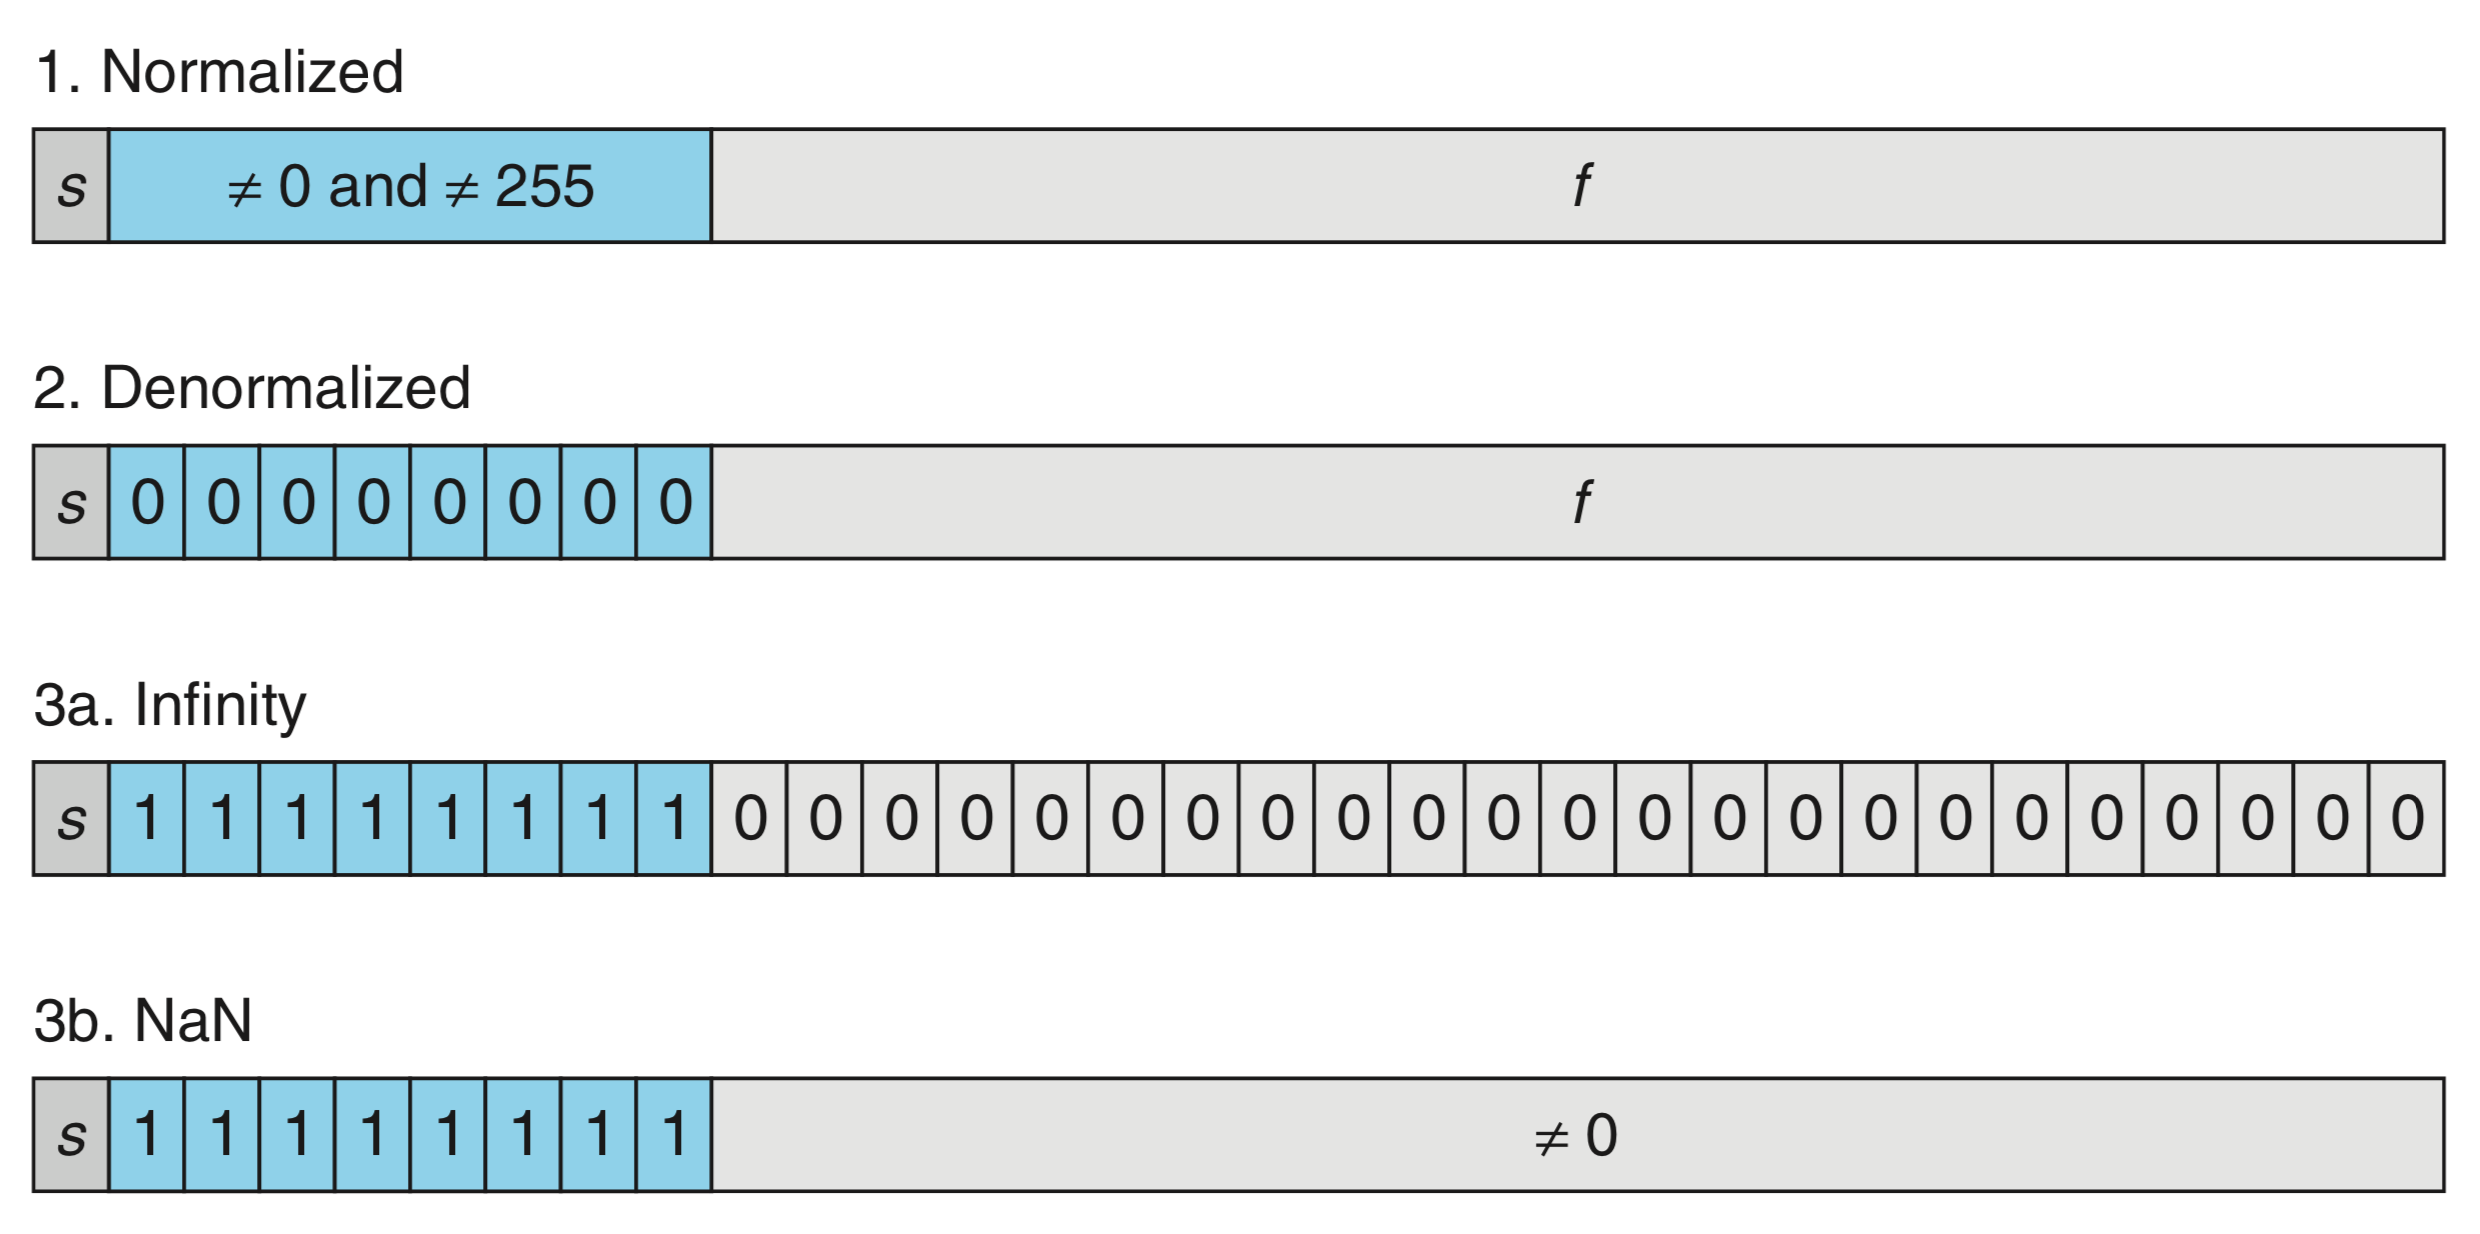
\includegraphics[width=0.9\textwidth]{figures/float_cases.png}\hfill
    \caption{Cases of the IEEE 754 Floating Point Standard.}
    \label{fig:float_cases}
\end{figure}

\begin{figure}[!htb]
    \centering
    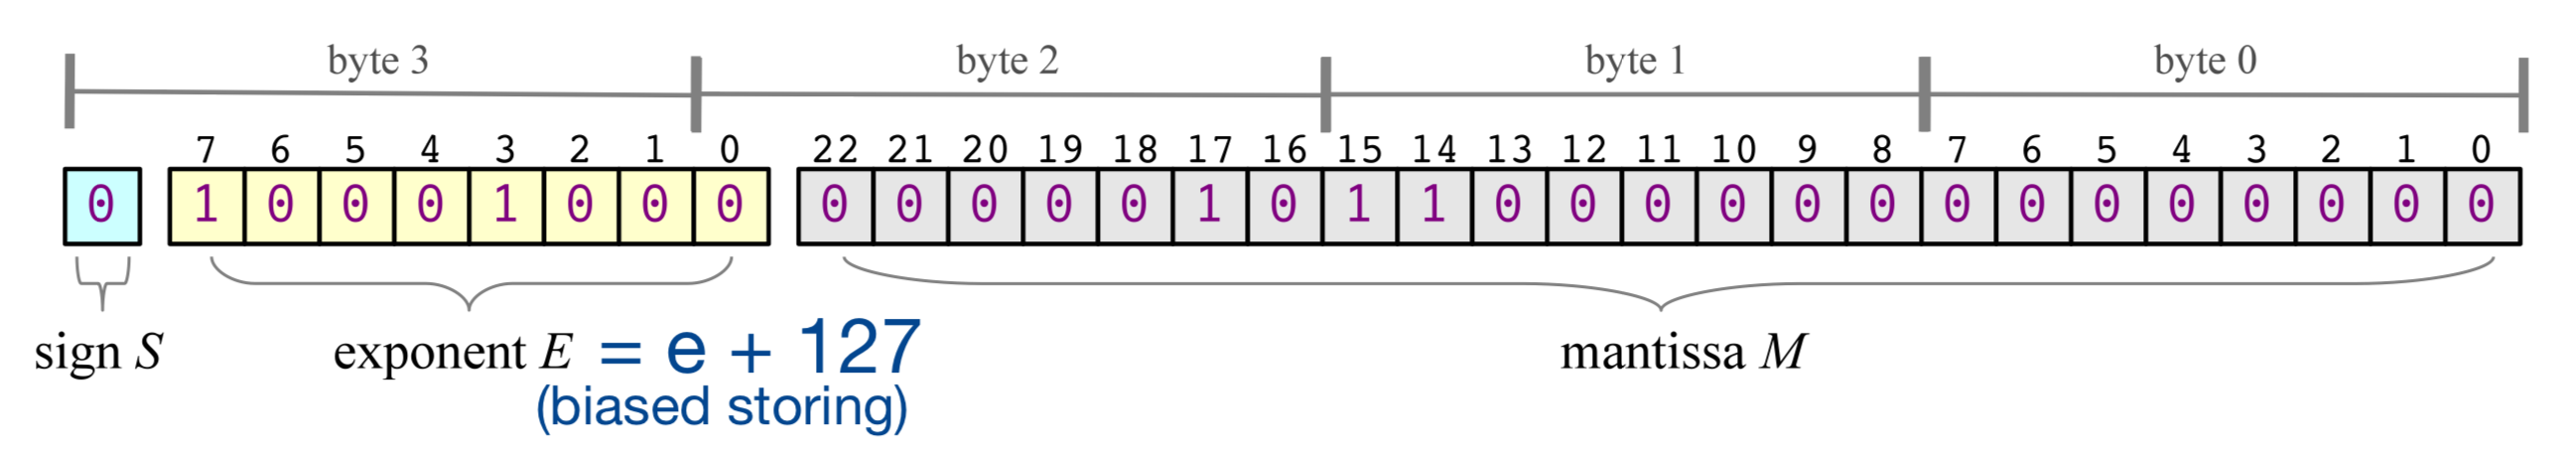
\includegraphics[width=0.9\textwidth]{figures/523float.png}\hfill
    \caption{523 can be written as $1.000001011_2 \cdot 2^9$ so $e=9, E = e + 127 = 136$. As of the normalization, the leading $1$ in the mantissa is implicit. The number is given as a single precision float in big endian.}
    \label{fig:523float}
\end{figure}

\subsubsection{Only a finite set of floating point numbers can be represented exactly}
With 32 bits, $2^{32}$ states can be encoded (and mind that here e.g. NaN has multiple representations). In any case,
the number of exactly representable numbers is finite, above $0$ starting at
\begin{equation}
    V_{\text{denorm,min}} = \frac{1}{2^p} \cdot 2^{-b+1} \explain{\approx}{single p.} 1.4 \cdot 10^{-45}
\end{equation}
with the smallest normalized number being
\begin{equation}
    V_{\text{norm,min}} = (1 + 0) \cdot 2^{-b} \explain{\approx}{single p.} 1.2 \cdot 10^{-38}
\end{equation}
and the largest normalized number being
\begin{equation}
    V_{\text{norm,max}} = (1 + \frac{2^p - 1}{2^p}) \cdot 2^{E_{\text{max}} - b} \explain{\approx}{single p.} 3.4 \cdot 10^{38}
\end{equation}

\subsubsection{Machine Precision is finite}
The smallest increment in the mantissa, in $1 + \frac{M}{2^p}$, is the \textbf{machine precision}
\begin{equation}
    \epsilon_{\text{mach}} = \frac{1}{2^p} \explain{\approx}{single p.} 1.2 \cdot 10^{-7}
\end{equation}
Consider two floating point numbers $V_1,V_2>0$ \textit{next to each other}
\begin{equation}
    V_1 = \left(1 + \frac{M}{2^p}\right) \cdot 2^{E - b}, \quad V_2 = \left(1 + \frac{M + 1}{2^p}\right) \cdot 2^{E - b}
\end{equation}
so their relative difference is bound by
\begin{equation}
    \frac{V_2 - V_1}{V_2} = \frac{\frac{1}{2^p} \cdot 2^{E - b}}{\left(1 + \frac{M + 1}{2^p}\right) \cdot 2^{E - b}} \leq \epsilon_{\text{mach}}
\end{equation}

\subsubsection{Rounding and Pitfalls of Floating Point Arithmetic}
In the IEEE standard, results of addition, subtraction, multiplication and division must equal to
one where the arithmetic operations are assumed to be exact and then there is rounding to the nearest
representable number (computation is done at higher (typically double or higher) precision). Therefore (mind the section before)
\begin{equation}
    \text{ralative error } \frac{|x-\hat{x}}{|x|} \leq \epsilon_{\text{mach}}, \quad \text{number } x, \text{ number on machine } \hat{x}
\end{equation}
with the common pitfalls
\begin{itemize}
    \item \textcolor{red1}{\textbf{Limitation of machine precision:}} $a+b=a$ typically for $|b| < \epsilon_{\text{mach}} |a|$, i.e. when $b$ cannot be resolved by the mantissa of $a$, e.g. $(1+0.5\epsilon) - 0.5\epsilon$ in floating point arithmetic yields $0.9999999999999999$ not $1$.
    \item \textcolor{red1}{\textbf{Associativity is not guarantueed:}} $(a+b)+c \explain{\ne}{i.A.} a+(b+c)$, e.g. $(2.3 + 1e20) - 1e20$ yields $0.0$ but $2.3 + (1e20 - 1e20)$ yields $2.3$
    \item \textcolor{red1}{\textbf{Problems of representability:}} As e.g. $0.1$ is not exactly representable in base $\beta = 2$, $x/10 \ne 0.1 \cdot x$ in general while $x/2.0 = 0.5 \cdot x$ is exact. The compiler may automatically choose the multiplication variant as multiplication is faster than division.
    \item \textcolor{red1}{\textbf{Cancellation:}} For $x = a - b$ subtractive cancellation causes relative errors already present in $\hat{a}$ and $\hat{b}$ to be (relatively) amplified, when $a$ and $b$ are of similar size. Significant digits are lost and the relative error explodes. Consider e.g. $a = 1.75682, b = 1.75471$ with $\hat{a} = 1.76$ and $\hat{b} = 1.75$. While $\hat{a},\hat{b}$ have small relative errors (3 digits precision\footnote{$\hat{x}$ is said to approximate $x$ to the r-th digit, if the absolute error is at most $\frac{1}{2}$ in the r-th digit, so 
    \begin{equation} \text{largest integer s so that } 10^s < |x|, \quad |x-\hat{x}| < 1/2 \cdot 10^{s-r+1} \end{equation}} Note that here $0.123$ ans $0.127$ agree in two significant digits, where one intuitively might say this should be rather $1$.), $a-b = 0.00211$ and $\hat{a} - \hat{b} = 0.01$ has a large relative error (no precise digit).
    \item \textcolor{red1}{\textbf{NaN and Inf:}} All calculations including NaN yield NaN, calculations with inf mostly inf (except of course 1/inf = 0, ...)
\end{itemize}
where we should
\begin{itemize}
    \item \textcolor{green1}{\textbf{Rewrite calculations so that errors do not amplify:}} For $x = 10^8, y = 10^5, z = - 1 - 10^5$ we have $xy+xz=-1.0066\cdot10^8$ (problem in resolving the $-1$ in $xz$) but $x(y+z) = -1.0\cdot10^8$.
    \item \textcolor{green1}{\textbf{Compare floats based on a maximum relative error:}} Instead of $x == y$ we should use e.g. $|x-y| \leq \epsilon_{\text{mach}} \cdot \max(|x|,|y|)$.
    \item \textcolor{green1}{\textbf{As avoid overflow to inf and nan:}} E.g. in \mintinline{C}{float x = 1e20; float y = x * x; float z = y / x} $z$ will be inf. 
\end{itemize}

\subsubsection{Rewriting Expressions to Avoid Cancellation I}
Consider $f(x) = \frac{1-\cos x}{x^2}$. For $x_e = 10^{-4}$, we have (when we represent 6 figures)
\begin{equation}
    c := \cos x_e, \quad \hat{c} = 0.999999, \quad 1-\hat{c} = 10^{-6}, \quad \text{while } 1-c \approx 5\cdot 10^{-9}
\end{equation}
$1-c$ has only one significant digit, the relative error is enormously amplified and we get
\begin{equation}
    \frac{1-\hat{c}}{x_e^2} = 100, \quad \text{ while in reality for } x\ne 0: 0 \leq f(x) \leq \frac{1}{2} 
\end{equation}
To avoid cancellation we can rewrite using $\cos x = \cos^2 \frac{x}{2} - \sin^2 \frac{x}{2} = 1 - 2 \sin^2 \frac{x}{2}$ to
\begin{equation}
    f(x) = \frac{1}{2} \left( \frac{\sin \frac{x}{2}}{\frac{x}{2}} \right)^2
\end{equation}
A comparison of both versions in python can be found in figure \ref{fig:cancellation_ex}, at some point (roughly below $10^{-8})$, $\cos x$ is too close to $1$ to be resolved by the mantissa, so the total result is $0$, above that the magnified error is visible.

\begin{figure}[!htb]
    \centering
    \includesvg[width=0.9\textwidth]{figures/canc.svg}\hfill
    \caption{Comparison of the mathematically equivalent expressions $f(x) = \frac{1-\cos x}{x^2}$ and $f(x) = \frac{1}{2} \left( \frac{\sin \frac{x}{2}}{\frac{x}{2}} \right)^2$ in python.}
    \label{fig:cancellation_ex}
\end{figure}

\subsubsection{Rewriting Expressions to Avoid Cancellation II}
Consider the following expressions for the sample variance of $\{x_i\}_{i=1}^N$
\begin{equation}
    \begin{multlined}
        \text{two-pass formula: } \bar{x} = \frac{1}{N} \sum_{i=1}^{N-1} x_i, \quad \sigma^2_N = \frac{1}{N} \sum_{i=1}^N (x_i - \bar{x})^2 \\ \text{one-pass formula: } \sigma^2_N = \frac{1}{N} \left( \sum_{i=1}^N x_i^2 - \frac{1}{N} \left( \sum_{i=1}^N x_i \right)^2 \right) \\ \text{ as } \sigma^2 = E[(x-\bar{x})^2] = E[x^2] - E[x]^2
    \end{multlined}
\end{equation}
While for the one-pass formula, we can calculate all necessary sums in one pass through the data, it suffers heavily from cancellation: For $\{10000,10001,10002\}$, the two-pass formula in single precision correctly gives $1.0$ while the one-pass formula yields $0.0$ (cancellation) (there are better one-pass formulas though).

\subsubsection{Accumulation of Round-off Errors}
Consider the sum
\begin{equation}
    \sum_{k=1}^\infty k^{-2} = \frac{\pi^2}{6}
\end{equation}
which we want to approximate by finitely many summands. If we sum the terms
just as the formula suggests from large to small, at some point, the small changes will not be resolved anymore - so better
sum up from small to large. Summing up in single precision for $N=10^7$ terms, one gets
\begin{equation}
    \begin{multlined}
        \text{big to small: } 1.644725323, \quad \text{small to big: } 1.644933939, \\ \text{exact (till 9th digit): } 1.644934058
    \end{multlined}
\end{equation}
As expected the big-to-small summation is too small.

\subsubsection{Higher Precision}
The above pitfalls are less severe in higher precision. For instance in double precision ($64$-bit)
\begin{equation}
    \begin{multlined}
        p = 52(+1) \text{ mantissa bits}, \quad 11 \text{ exponent bits, with } e_{min} = -1022, e_{max} = 1023,\\ \text{ smallest and largest repr. numbers } f_{min} \simeq 2.2 \cdot 10^{-308}, f_{max} \simeq 1.8 \cdot 10^{308},\\ |e_{min}| < |e_{max}| \rightarrow \frac{1}{f_{min}} < f_{max}
    \end{multlined}
\end{equation}
with machine precision $\epsilon_{\text{mach}} \approx 2.2 \cdot 10^{-16}$. There is even quad-double precision ($128$-bit) (not supported on hardware though and therefore relatively slow as it has to be emulated). Packages for nearly arbitrary precision also exist.

\subsection{A more general view on sources of numerical error}
In numerical computation, the typical error sources are
\begin{itemize}
    \item rounding
    \item data uncertainty
    \item truncation (of terms in numerical schemata, e.g. in the approximation of a function by its Taylor series)
\end{itemize}
where we have now discussed rounding errors and their effects to some extent.

\subsection{Backward error, forward error and condition number}
Consider we approximate $y=f(x)$ as $\hat{y}$ in an arithmetic of limited precision, with $f: \mathbb{R} \rightarrow \mathbb{R}$.
\begin{itemize}
    \item \textbf{Forward error:} The absolute or relative error between $\hat{y}$ and $y$ is the forward error (living in the output space)
    \item \textbf{Backward error:} The backward error is the smallest $\Delta x$ (in the input space) so that $f(x+\Delta x) = \hat{y}$, so the smallest perturbation where the exact function gives our approximate result.
\end{itemize}
If this $\Delta x$ is sufficiently small, e.g. as small as the uncertainty in the data in the first place, we speak
of backward stability. A weaker formulation is the mixed forward-backward error
\begin{equation}
    \hat{y} + \Delta y = f(x + \Delta x), \quad |\Delta y| \leq \epsilon |y|, \quad |\Delta x| \leq \eta |x|
\end{equation}
In the context of rounding errors, we call the algorithm numerically stable if $\hat{y}$ is almost the right answer for
almost the right data ($\epsilon,\eta$ small).
\subsubsection{Conditioning}
Backward and forward error are connected by the conditioning of a problem, the sensitivity of the
solution to perturbations in the data. Assuming $\hat{y} = f(x + \Delta x)$ and $f$ differentiable, we have
\begin{equation}
    \hat{y} - y = f(x + \Delta x) - f(x) = f'(x) \Delta x + \mathcal{O}((\Delta x)^2)
\end{equation}
so the relative error is
\begin{equation}
    \frac{\hat{y} - y}{y} = \frac{f'(x) \Delta x}{f(x)} + \mathcal{O}((\Delta x)^2)
\end{equation}
leading to the relative condition number
\begin{equation}
    \kappa(x) \explain{=}{i.A.} \lim_{\epsilon \rightarrow 0^+} \sup_{||\Delta x|| \leq \epsilon} \frac{||y-\hat{y}|| / ||y||}{||\Delta x|| / ||x||} = \left| \frac{x f'(x)}{f(x)} \right|
\end{equation}
for small $\Delta x$ measuring the relative change in the output over a relative change in the input.
As a rule of thumb
\begin{equation}
    \text{forward error } \lesssim \text{condition number } \cdot \text{ backward error}
\end{equation}
so ill-conditioned problems can have large forward errors.

\textbf{Application on Matrices}\par
Consider the linear system $\mat{A}\vec{y}=\vec{x}, \vec{y} = \mat{A}^{-1}\vec{x}, \vec{\hat{y}} = \mat{A}^{-1}(\vec{x} + \vec{\Delta x})$. The condition number follows as
\begin{equation}
    \begin{aligned}
        \kappa(\mat{A}) &= \max_{\vec{x},\vec{\Delta x} \ne 0} \frac{||\mat{A}^{-1}\vec{x}-\mat{A}^{-1}(\vec{x} + \vec{\Delta x})|| / ||\mat{A}^{-1}\vec{x}||}{||\vec{\Delta x}|| / ||\vec{x}||} \\
                        &= \max_{\vec{\Delta x} \ne 0} \frac{||\mat{A}^{-1}\vec{\Delta x}||}{||\Delta x||} \max_{\vec{x} \ne 0} \frac{||\vec{x}||}{||\mat{A}^{-1}\vec{x}||} \\
                        &= \max_{\vec{\Delta x} \ne 0} \frac{||\mat{A}^{-1}\vec{\Delta x}||}{||\vec{\Delta x}||} \max_{\vec{y} \ne 0} \frac{||\mat{A}\vec{y}||}{||\vec{y}||} \\
                        &= ||\mat{A}^{-1}|| \cdot ||\mat{A}||
    \end{aligned}
\end{equation}
where we used the definition of the matrix norm $||\mat{A}|| = \max_{\vec{x} \ne 0} \frac{||\mat{A}\vec{x}||}{||\vec{x}||}$. For large condition numbers, small perturbations in the input $\vec{x}$ lead to
large changes in the solution $\vec{y}$.
    
